\documentclass{article}

% Language setting
% Replace `english' with e.g. `spanish' to change the document language
\usepackage[italian]{babel}

% Set page size and margins
% Replace `letterpaper' with`a4paper' for UK/EU standard size
\usepackage[letterpaper,top=2cm,bottom=2cm,left=3cm,right=3cm,marginparwidth=1.75cm]{geometry}

% Useful packages
\usepackage{listings}
\usepackage{xcolor}
\usepackage[utf8]{inputenc}
\usepackage[shortlabels]{enumitem}
\usepackage{amsmath}
\usepackage{graphicx}
\usepackage[export]{adjustbox} 
\usepackage[colorlinks=true, allcolors=blue]{hyperref}

\definecolor{codegreen}{rgb}{0,0.6,0}
\definecolor{codegray}{rgb}{0.5,0.5,0.5}
\definecolor{codepurple}{rgb}{0.58,0,0.82}
\definecolor{backcolour}{rgb}{0.95,0.95,0.92}

\lstdefinestyle{javastyle}{
    backgroundcolor=\color{backcolour},   
    commentstyle=\color{codegreen},
    keywordstyle=\color{magenta},
    numberstyle=\tiny\color{codegray},
    stringstyle=\color{codepurple},
    basicstyle=\ttfamily\footnotesize,
    breakatwhitespace=false,         
    breaklines=true,                 
    captionpos=b,                    
    keepspaces=true,                 
    numbers=left,                    
    numbersep=5pt,                  
    showspaces=false,                
    showstringspaces=false,
    showtabs=false,                  
    tabsize=2
}

\lstdefinestyle{bashstyle}{
    backgroundcolor=\color{backcolour},   
    commentstyle=\color{codegreen},
    keywordstyle=\color{magenta},
    numberstyle=\tiny\color{codegray},
    stringstyle=\color{codepurple},
    basicstyle=\ttfamily\footnotesize,
    breakatwhitespace=false,         
    breaklines=true,                 
    captionpos=b,                    
    keepspaces=true,                 
    showspaces=false,                
    showstringspaces=false,
    showtabs=false
}

\lstdefinestyle{bashstyle_table}{
    commentstyle=\color{codegreen},
    keywordstyle=\color{magenta},
    numberstyle=\tiny\color{codegray},
    stringstyle=\color{codepurple},
    basicstyle=\ttfamily\footnotesize,
    breakatwhitespace=false,         
    breaklines=true,                 
    captionpos=b,                    
    keepspaces=true,                 
    showspaces=false,                
    showstringspaces=false,
    showtabs=false
}

\title{Basi di dati - EasyRegatta}
\author{Antonio Marini - 559200}

\begin{document}
\maketitle
\newpage

\section{Descrizione del dominio.}

\begin{flushleft}
Si vuole costruire un sistema che permette a una Autorità organizzatrice,
di creare e gestire regate, per la precisione regate di flotta.
\end{flushleft}

\begin{flushleft}
L'Autorità potrà creare un catalogo di bandi. Un bando sarà sempre relativo a una regata e viceversa. 
\end{flushleft}

\begin{flushleft}
Un equipaggio che intende iscriversi a un bando con una barca, dovrà comunicare la classe della barca, che, se non presente tra la lista di classi ammissibili del bando , verrà rifiutata.
\end{flushleft}

\begin{flushleft}
Il sistema mantiene tutte le comunicazioni fatte per ogni regata tenuta nella storia.
All' interno di una regata ci sono diversi tipi e sottotipi di comunicazioni fattibili tra barche e comitato.
Le principali tre (3 insiemi copertura di comunicazioni) sono: 
\begin{itemize}
    \item Passaggi alle boe: vengono comunicate dalle barche che passano una determinata boa, 
    \item Avvisi: vengono fatte dal comitato verso le varie barche. Rimpiazzano le classiche bandiere.
    \item Proteste: vengono fatte da barche verso altre barche, giudicabili negative o positive dal comitato a posteriori.
\end{itemize}
Sia le barche partecipanti che la barca comitato avranno una postazione con un terminale che si interfaccia al sistema, permettendo al membro dell'equipaggio o del comitato di creare la comunicazione.
Il comitato può scegliere se iniziare il processo di partenza per una certa barca, e quindi comunicare i 3 Segnali per la partenza impostando i tempi.
Sempre il comitato può, dall'interfaccia, visualizzare le proteste fatte durante la regata, esprimendo un giudizio (positivo o negativo) e i punti di penalità da detrarre alla barca protestata.
Gli equipaggi invece avranno un'interfaccia diversa, con la possibilità di inserire un nuovo passaggio alla boa, o inviare una protesta che poi verrà esaminata dal comitato.
\end{flushleft}

\begin{flushleft}
Per poter costruire la classifica finale della regata, il comitato dall'applicazione chiederà di calcolare la classifica scegliendo se si vuole tener conto anche di chi non e riuscito ad arrivare all'arrivo nel tempo limite.
La vista conterrà, per ogni barca, i nomi degli equipaggi, i numeri velici della barca, la somma di tutte le penalità ricevute con proteste(giudicate positive), il tempo finale di arrivo (alla boa 10), e un punteggio calcolato con una certa formula seguendo le istruzioni pubblicate dal comitato che tiene conto sia dei tempi che delle proteste ricevute.
\end{flushleft}

\begin{flushleft}
Per i bandi bisogna tenere informazioni sulla data in cui si tiene.\newline
Un bando deve poter ammettere una o più classi di barche.
Una classe di barche può essere ammessa in zero, una o più bandi.
\end{flushleft}

\begin{flushleft}
Una barca deve possedere solo una classe.
Una classe può essere relativa 0, uno o più  barche.
\end{flushleft}

\begin{flushleft}
Una barca può iscriversi a zero, uno o più bandi solo se la sua classe appartiene alla lista di classi ammesse del bando di regata.\newline
A un bando possono iscriversi una o più barche.\newline
Una barca che intende ritirarsi dovrà ritirare (cancellare) iscrizione nel bando entro 48 ore dalla data della regata. In caso di mancato avviso verrà squalificata per i prossimi 30 giorni, non potendo più partecipare ad alcuna regata organizzata dall'Autorità.
L'attributo giorni\_squalifica indica il numero di giorni di squalifica della barca. 
\end{flushleft}

\begin{flushleft}
Un bando rappresenta un modello di una regata che si terrà.
Una regata infatti corrisponde sempre a un solo bando. Un bando corrisponde a una sola regata. Non può esistere una regata senza bando, mentre invece un bando può non essere reso a una regata per esempio, perché il numero di partecipanti è troppo basso.
\end{flushleft}

\begin{flushleft}
Una barca deve possedere un solo equipaggio.
Un equipaggio può far parte di una sola barca.
L'equipaggio assieme a tutti i suoi membri verranno iscritti automaticamente quando viene iscritta la barca relativa.
\end{flushleft}

\begin{flushleft}
Il sistema mantiene riferimento alle persone, coi loro nominativi, numero di tessera, e codice fiv. Si avrà una superclasse copertura di persone che comprende le sottoclassi Commissari e Partecipanti.
\end{flushleft}

\begin{flushleft}
Un equipaggio è formato da più partecipanti.
Un partecipante deve essere membro di un solo equipaggio.
\end{flushleft}

\begin{flushleft}
Un comitato crea istruzioni per la regata, e giudica le proteste delle barche partecipanti.
Le istruzioni sono volutamente state semplificate ad attributo e non a classe con i vari valori nel dettaglio. 
Non possono mai esserci comitati uguali per regata, anche se formati dagli stessi commissari, avranno sempre un id diverso ogni volta che vengono scelti dall'Autorità organizzatrice.
Un comitato deve condurre una sola regata.
Una regata deve essere condotta da un solo comitato.
\end{flushleft}

\begin{flushleft}
Un comitato deve essere formato da uno o più commissari.
Un commissario può far parte di un solo comitato.
\end{flushleft}

\begin{flushleft}
Una protesta deve avere una barca protestante e una barca protestata.
Una barca può essere una barca protestante o protestata in una o più proteste.
\end{flushleft}

\begin{flushleft}
Un segnale deve essere mandato a un solo equipaggio.
Un equipaggio deve ricevere più segnali (3).
\end{flushleft}

\begin{flushleft}
Un equipaggio può comunicare uno o più passaggi alle boe.
Un passaggio alle boe deve essere relativo a un unico equipaggio.
\end{flushleft}

\subsection{Classi trovate}

Sono state individuate \textbf{13 Classi.}

\begin{itemize}
    \item \textbf{Bandi}: rappresenta l'insieme dei bandi disponibili dell'organizzazione
    \item \textbf{Barche}: rappresenta l'insieme di barche profilate che si sono iscritte a dei bandi nella storia.
    \item \textbf{Classi}: rappresenta l'insieme di classi generali che una barca può avere.
    \item \textbf{Regate}: rappresenta l'insieme delle regate (eventi) relative ai bandi.
    \item \textbf{Equipaggi}: rappresenta l'insieme degli equipaggi registrati nelle barche.
    \item \textbf{Partecipanti}: rappresenta l'insieme di tutti i partecipanti che fanno parte di un equipaggio iscritti ai bandi. Sottoclasse di Persone.
    \item \textbf{Comitati}: Rappresenta l'insieme dei comitati scelti.
    \item \textbf{Commissari}: Rappresenta l'insieme di persone che fanno parte di una commissione. Sottoclasse di Persone.
    \item \textbf{Persone}: Superclasse che rappresenta l'insieme di tutte le persone.
    \item \textbf{Proteste}: L'insieme di proteste fatte da barche verso altre. Sottoclasse copert. di comunicazioni.
    \item \textbf{Segnali}: L'insieme di Segnali. Sottoclasse copert. di Comunicazioni.
    \item \textbf{PassaggiBoe}: L'insieme dei passaggi di boa. Sottoclasse copert. di Comunicazioni.
    \item \textbf{Comunicazioni}: L'insieme delle comunicazioni fatte in un certo tempo.
\end{itemize}

\section{Schema concettuale.}
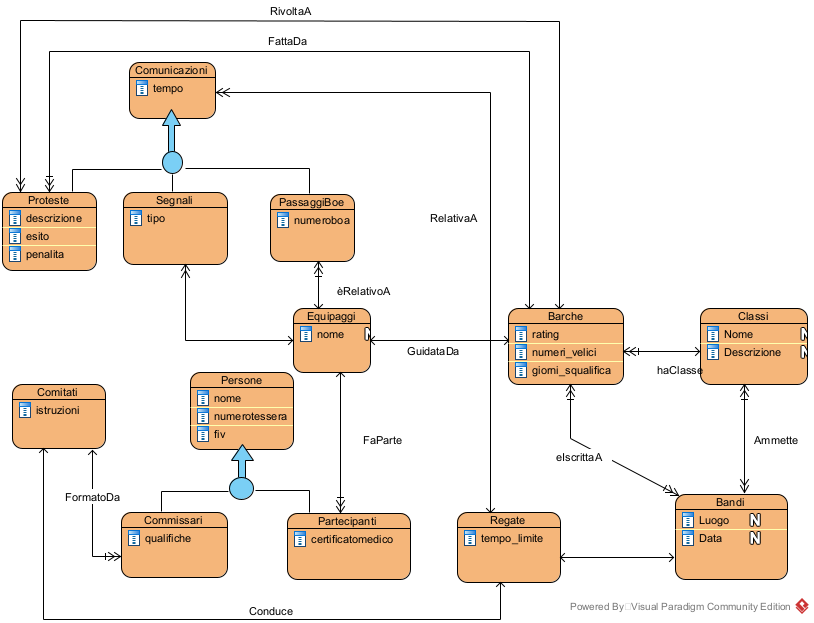
\includegraphics[max size={\textwidth}{\textheight}]{concettuale.png}

\newpage
\subsection{Vincoli intrarelazionali.}

\begin{itemize}
    \item Ogni classe ha un attributo \textbf{id\_[nome\_entita]} come \textbf{PRIMARY KEY}. 
    \item Tutti gli attributi sono intesi come \textbf{NOT NULL} a parte la descrizione delle Classi.
    \item L'attributo \textbf{fiv} di Persone deve avere \textbf{esattamente 11 catatteri}
    \item L'attributo \textbf{numero\_tessera} di Persone deve avere \textbf{esattamente 6 catatteri}
    \item L'attributo \textbf{istruzioni} di Comitati deve avere \textbf{meno di 500 caratteri}.
    \item L'attributo \textbf{numeri\_velici} di Barche deve avere \textbf{esattamente 10 cifre}.
    \item L'attributo \textbf{numero\_boa} di PassaggiBoe deve essere \textbf{compreso tra 1 e 10}.
    \item L'attributo \textbf{penalita} di Proteste deve essere \textbf{compreso tra 1 e 25}.
    \item L'attributo \textbf{tipo} di Segnali può essere un valore compreso nel dizionario \\
    di valori \textbf{['Avviso', 'Ultimo Minuto', 'Partenza']} dove ognuno di essi dovrà avere tempo maggiore del precedente.\\
    In particolare la dfferenza di tempo tra 'Avviso' e 'Ultimo Minuto' sarà di 4 minuti, 
    mentre sarà di 1 minuto tra 'Ultimo Minuto' e 'Partenza'.
    
\end{itemize}

\subsection{Vincoli interrelazionali}

\begin{itemize}
    \item L'attributo \textbf{tempo} di \textbf{Segnali} per un equipaggio deve essere sempre minore dei tempi nei passaggi alle boe di quell'equipaggio.
    \item Per poter considerare una barca arrivata in tempo, la differenza \\tra l'attributo \textbf{tempo} di \textbf{PassaggiBoe} alla boa numero 10 per quella barca, e l'attributo \textbf{tempo} in \textbf{Segnali} di tipo 'Partenza', deve essere minore dell'attributo \textbf{tempo\_limite} di Regate.
\end{itemize}

\newpage
\section{Schema logico relazionale.}

\subsection{Formato testuale.}

\begin{itemize}
    \item \textbf{Bandi}(\underline{id\_bando}, luogo, data)
    \item \textbf{Regate}(\underline{id\_regata}, tempo\_limite, bando*, comitato*)
    \item \textbf{Classi}(\underline{id\_classe}, nome, descrizione)
    \item \textbf{ClassiBandi}(\underline{id\_bando*}, \underline{id\_classe*})
    \item \textbf{Barche}(\underline{id\_barca}, rating, numeri\_velici, giorni\_squalifica, equipaggio*, classe*)
    \item \textbf{BarcheBandi}(\underline{id\_barca*}, \underline{id\_bando*})
    \item \textbf{Equipaggi}(\underline{id\_equipaggio}, nome)
    \item \textbf{Persone}(\underline{id\_persona}, fiv, numero\_tessera, nome)
    \item \textbf{Partecipanti}(\underline{id\_persona*}, certificato\_medico, equipaggio*)
    \item \textbf{Commissari}(\underline{id\_persona*}, qualifiche, comitato*)
    \item \textbf{Comunicazioni}(\underline{id\_comunicazione*}, tempo)
    \item \textbf{Proteste}(\underline{id\_comunicazione*}, descrizione, esito, penalita, barca\_protestante*, \newline barca\_contestata*)
    \item \textbf{Segnali}(\underline{id\_comunicazione*}, tipo, equipaggio*)
    \item \textbf{PassaggiBoe}(\underline{id\_comunicazione*}, numero\_boa, equipaggio*)
\end{itemize}

\subsection{Dipendenze funzionali.}

Tutte le relazioni soddisfano la forma normale di Boyce-Codd, ovvero in tutte le relazioni si verifica:\\
Per ogni dipendenza $X \rightarrow A$ appartenenti a F, non banali, X e una superchiave.\\
Questo puo essere verificato facilmente utilizzando l'algoritmo di Analisi per tutte le relazioni e rispettivi insiemi di dipendenze, che come detto prima ne comprenderanno solo una \\
$F = \{id\_[nome\_relazione] \rightarrow resto degli attributi\}.$

\subsection{Formato grafico.}

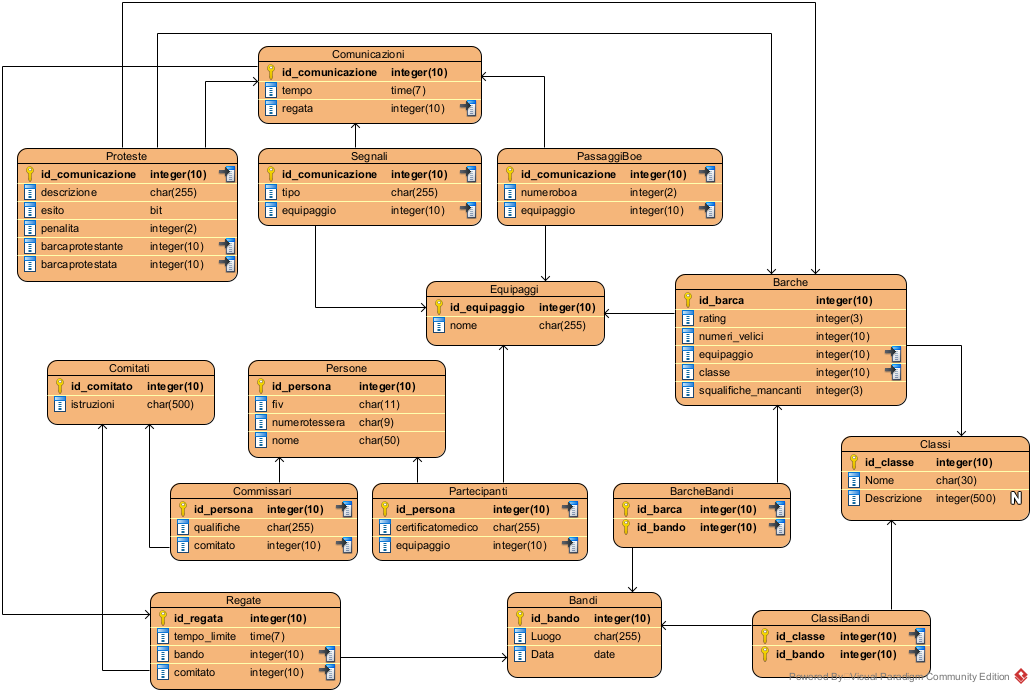
\includegraphics[max size={\textwidth}{\textheight}]{logico.png}

\section{Query SQL.}

\begin{enumerate}[a)]
    \item Nome dell'equipaggio, numeri velici, nome della classe delle barche che sono iscritte al bando in data 23-08-2021. 
    
    \lstset{style=bashstyle}
    \begin{lstlisting}[language=sql]
    
        SELECT e.nome as 'Nome Equipaggio' , 
               bc.numeri_velici as 'Numeri Velici', 
               c.nome as 'Classe', 
        FROM Classi c 
            JOIN Barche bc ON (bc.classe = c.id_classe) 
            JOIN Equipaggi e ON (bc.equipaggio = e.id_equipaggio) 
            JOIN BarcheBandi bb ON (bc.id_barca = bb.id_barca) 
            JOIN Bandi ba ON (bb.id_bando = ba.id_bando)
        WHERE ba.data = '23-08-2021'
    \end{lstlisting} 
    
    \item Per ogni classe di barche che hanno più di 3 barche di quella classe e senza giorni di squalifica indicare rating minimo e rating massimo, ordinandole per numero di barche di quella classe crescente.
    
    \lstset{style=bashstyle}
    \begin{lstlisting}[language=sql]
    
        SELECT MIN(rating) as 'Rating minimo',
               MAX(rating) as 'Rating massimo' 
        FROM Classi c JOIN Barche bc ON (bc.classe = c.id_classe) 
        WHERE bc.giorni_squalifica = 0
        GROUP BY bc.classe HAVING count(*) > 3
        ORDER BY count(*)
        
    \end{lstlisting} 
    
    \newpage
    \item Per ogni barca che ha ricevuto piu' di 3 proteste, il numero di proteste positive ricevute.
    
    \lstset{style=bashstyle}
    \begin{lstlisting}[language=sql]
    
        SELECT count(*) as 'Numero Proteste Ricevute'
        FROM Proteste p JOIN Barche bc ON (p.barca_contestata=bc.id_barca)
        WHERE p.esito = 1
        GROUP BY p.barca_contestata HAVING count(*) > 3
        
    \end{lstlisting}
    
    \item Nome equipaggio e numeri velici delle barche che hanno ricevuto almeno una protesta con penalita maggiore di 10.
    
    \lstset{style=bashstyle}
    \begin{lstlisting}[language=sql]
    
        SELECT bc.numeri_velici as 'Numeri Velici',
               e.nome as 'Nome Equipaggio'
        FROM Equipaggi e JOIN Barche bc ON (e.id_equipaggio = bc.equipaggio)
        WHERE EXISTS  (SELECT * 
                        FROM Proteste p
                        WHERE p.barca_contestata = bc.id_barca 
                        AND p.penalita > 10)
        
    \end{lstlisting} 
    
    \item Indicare numeri velici, nome dell'equipaggio, delle barche che hanno presentato proteste sempre con esito positivo. (per esito positivo si intende esito = 1)
    
    \lstset{style=bashstyle}
    \begin{lstlisting}[language=sql]
    
        SELECT bc.numeri_velici as 'Numeri Velici',
               e.nome as 'Nome Equipaggio'
        FROM Equipaggi e JOIN Barche bc ON (e.id_equipaggio = bc.equipaggio)
        WHERE NOT EXISTS (SELECT * 
                        FROM Proteste p
                        WHERE p.barca_protestante = bc.id_barca 
                        AND p.esito = 0)
        
    \end{lstlisting}
    
    \item Indicare nome degli equipaggi delle barche che sono arrivati dopo il tempo prestabilito in almeno una regata. \newline(arrivo = boa 10).
    
    \lstset{style=bashstyle}
    \begin{lstlisting}[language=sql]
    
    SELECT e.nome as 'Nome equipaggio'
    FROM Equipaggi e
    WHERE e.id_equipaggio 
            =ANY (SELECT e2.id_equipaggio
                  FROM  Regate r 
                        JOIN Comunicazioni c ON (c.regata = r.id_regata)
                        JOIN PassaggiBoe pb USING(id_comunicazione)
                        JOIN Segnali s USING(id_comunicazione)
                        JOIN Equipaggi e2 ON (pb.equipaggio = e2.equipaggio)
                  WHERE pb.numero_boa = 10 AND a.tipo = 'Partenza' AND pb.tempo - a.tempo > r.tempo_limite
                )
    
    \end{lstlisting}
    
\end{enumerate}

\newpage
\section{Piani di accesso.}
\subsection{Piani di accesso logico.}

\subsubsection{QUERY a)}
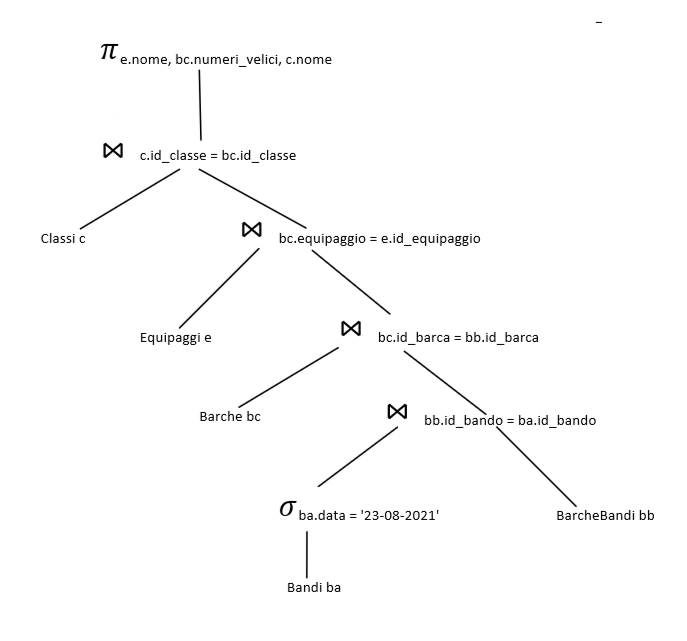
\includegraphics[]{logicoa.png}

\subsubsection{QUERY b)}
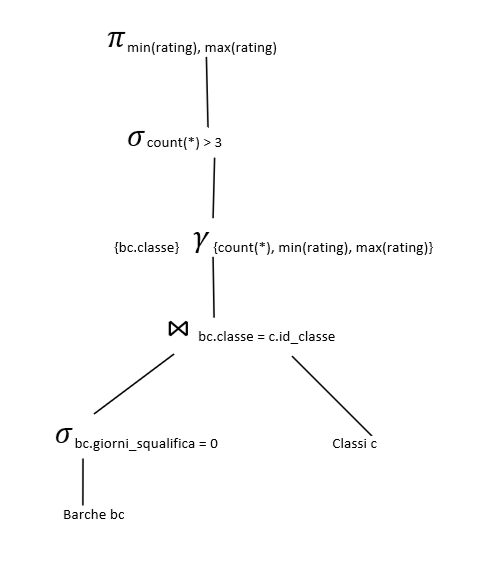
\includegraphics[]{logicob.png}

\subsubsection{QUERY c)}
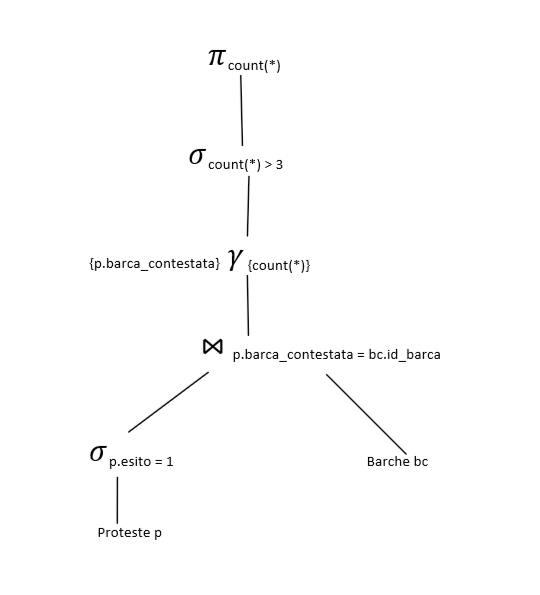
\includegraphics[]{logicoc.png}

\subsection{Piani di accesso fisico(senza indici)}

\subsubsection{QUERY a)}
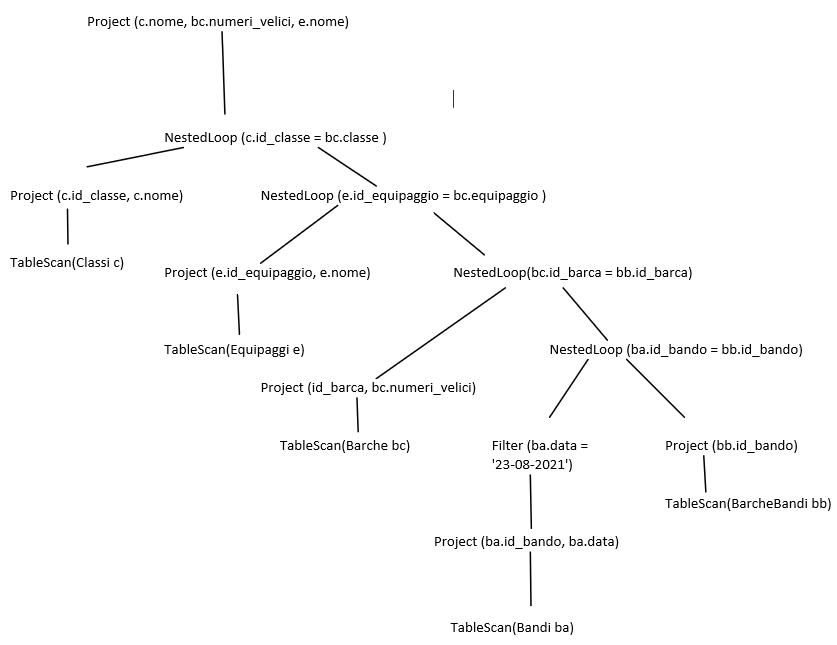
\includegraphics[]{fisicoa.png}

\subsubsection{QUERY b)}
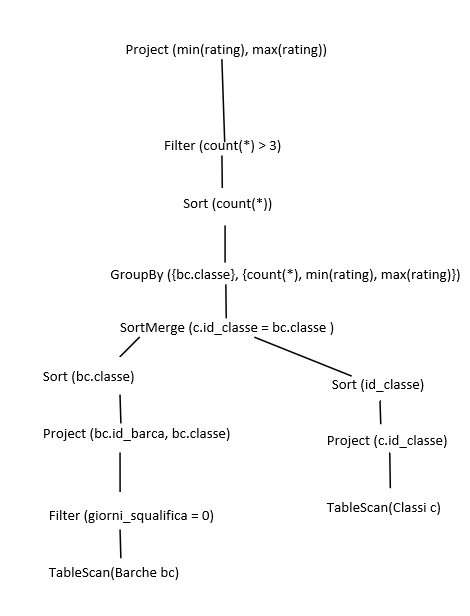
\includegraphics[]{fisicob.png}

\subsubsection{QUERY c)}
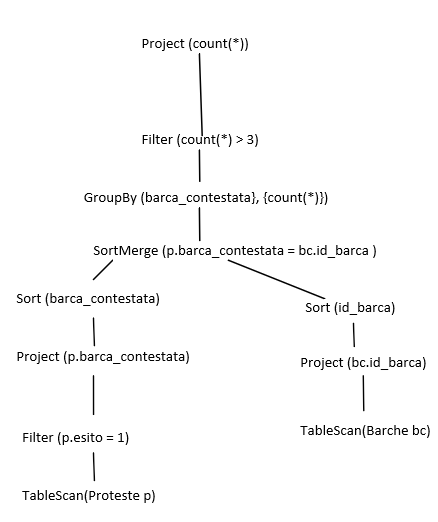
\includegraphics[]{fisicoc.png}

\subsection{Piani di accesso fisico(con indici)}

\subsubsection{QUERY a)}
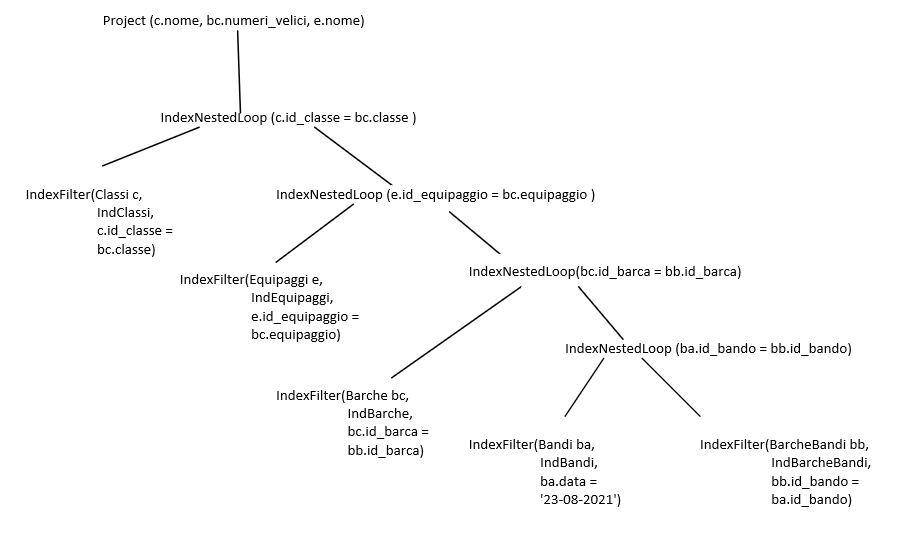
\includegraphics[]{fisicoinda.png}
\begin{flushleft}
INDICI 5:
\begin{itemize}
    \item \textbf{IndBandi} sulla tabella \textbf{Bandi} e attributo \textbf{data}
    \item \textbf{IndBarcheBandi} sulla tabella \textbf{BarcheBandi} e attributo \textbf{id\_bando}
    \item \textbf{IndBarche} sulla tabella \textbf{Barche} e attributo \textbf{id\_barca}
    \item \textbf{IndEquipaggi} sulla tabella \textbf{Equipaggi} e attributo \textbf{id\_equipaggio}
    \item \textbf{IndClassi} sulla tabella \textbf{Classi} e attributo \textbf{id\_classe}
\end{itemize}
\end{flushleft}

\subsubsection{QUERY b)}
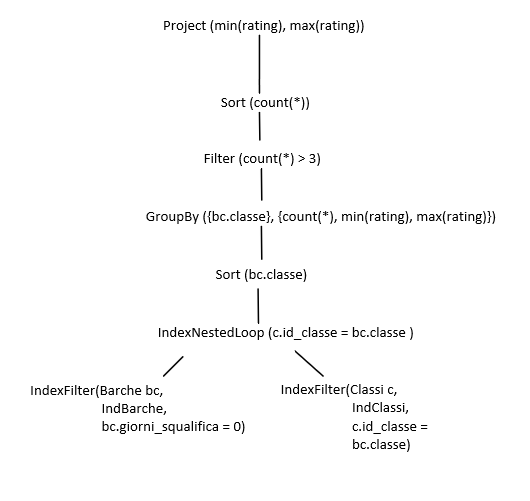
\includegraphics[]{fisicoindb.png}
\begin{flushleft}
INDICI 2:
\begin{itemize}
    \item \textbf{IndBarche} sulla tabella \textbf{Barche} e attributo \textbf{giorni\_squalifica}
    \item \textbf{IndClassi} sulla tabella \textbf{Classi} e attributo \textbf{id\_classe}
\end{itemize}
\end{flushleft}

\newpage
\subsubsection{QUERY c)}
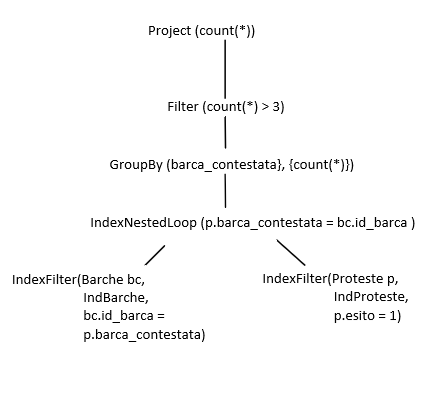
\includegraphics[]{fisicoindc.png}

\begin{flushleft}
INDICI 2:
\begin{itemize}
    \item \textbf{IndProteste} sulla tabella \textbf{Proteste} e attributo \textbf{esito}
    \item \textbf{IndBarche} sulla tabella \textbf{Barche} e attributo \textbf{id\_barca}
\end{itemize}
\end{flushleft}

\end{document}